\section{Problem 1-1 Adjacency Matrix}

\begin{enumerate}
	\item Is the corresponding graph G directed or undirected? Justify your answer.
	
	Undirected, because the adjacency matrix is symmetric.
	
	\item Draw the graph described by the adjacency matrix $A_G$. Use labels to indicate the correspondence of nodes to rows or columns of the adjacency matrix.
	
	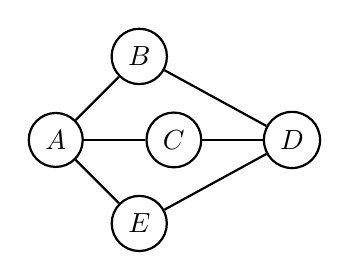
\begin{tikzpicture}[node distance={15mm}, thick, main/.style = {draw, circle}] 
	\node[main] (A) {$A$}; 
	\node[main] (B) [above right of=A] {$B$}; 
	\node[main] (C) [right of=A] {$C$};
	\node[main] (D) [right of=C] {$D$}; 
	\node[main] (E) [below right of=A] {$E$};
	\draw (A) -- (B);
	\draw (A) -- (C);
	\draw (A) -- (E);
	\draw (B) -- (D);
	\draw (C) -- (D);
	\draw (E) -- (D);
	\end{tikzpicture} 
	
	\item Is the graph bipartite? Explain your answer by giving 2-3 sentences.
	
	Yes, the graph is bipartite. It can be divided into the two disjoint sets $U = {A, D}$ and $V = {B, C, E}$. The nodes connect these two sets, but never connect two nodes in one set (independent set property).
	
	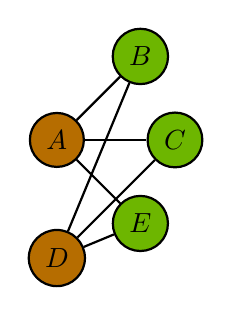
\begin{tikzpicture}[node distance={15mm}, thick, main/.style = {draw, circle}] 
	\node[main, fill={rgb:red,4;green,2;yellow,1}] (A) {$A$}; 
	\node[main, fill={rgb:red,2;green,4;yellow,1}] (B) [above right of=A] {$B$}; 
	\node[main, fill={rgb:red,2;green,4;yellow,1}] (C) [right of=A] {$C$};
	\node[main,fill={rgb:red,4;green,2;yellow,1}] (D) [below of=A] {$D$}; 
	\node[main, fill={rgb:red,2;green,4;yellow,1}] (E) [below right of=A] {$E$};
	\draw (A) -- (B);
	\draw (A) -- (C);
	\draw (A) -- (E);
	\draw (B) -- (D);
	\draw (C) -- (D);
	\draw (E) -- (D);
	\end{tikzpicture} 
	
	\item Give the adjacency list and the edge list representation of the graph G.
	
	adjacency list:
	
	\begin{tabular}{ | m{3cm} | m{3cm} | } 
		\hline
		node & linked to \\ 
		\hline
		A & B, C, E \\ 
		\hline
		B & A, D \\ 
		\hline
		C & A, D \\ 
		\hline
		D & B, C, E \\ 
		\hline
		E & A, D \\ 
		\hline
	\end{tabular}

	edge list:

	\begin{tabular}{ | m{3cm} | m{3cm} | } 
		\hline
		pair of edges \\ 
		\hline
		(A, B) \\ 
		\hline
		(A, C) \\ 
		\hline
		(A, E) \\ 
		\hline
		(B, D) \\ 
		\hline
		(C, D) \\ 
		\hline
		(D, E) \\ 
		\hline
	\end{tabular}
	
\end{enumerate}